% Oscilloscope grid
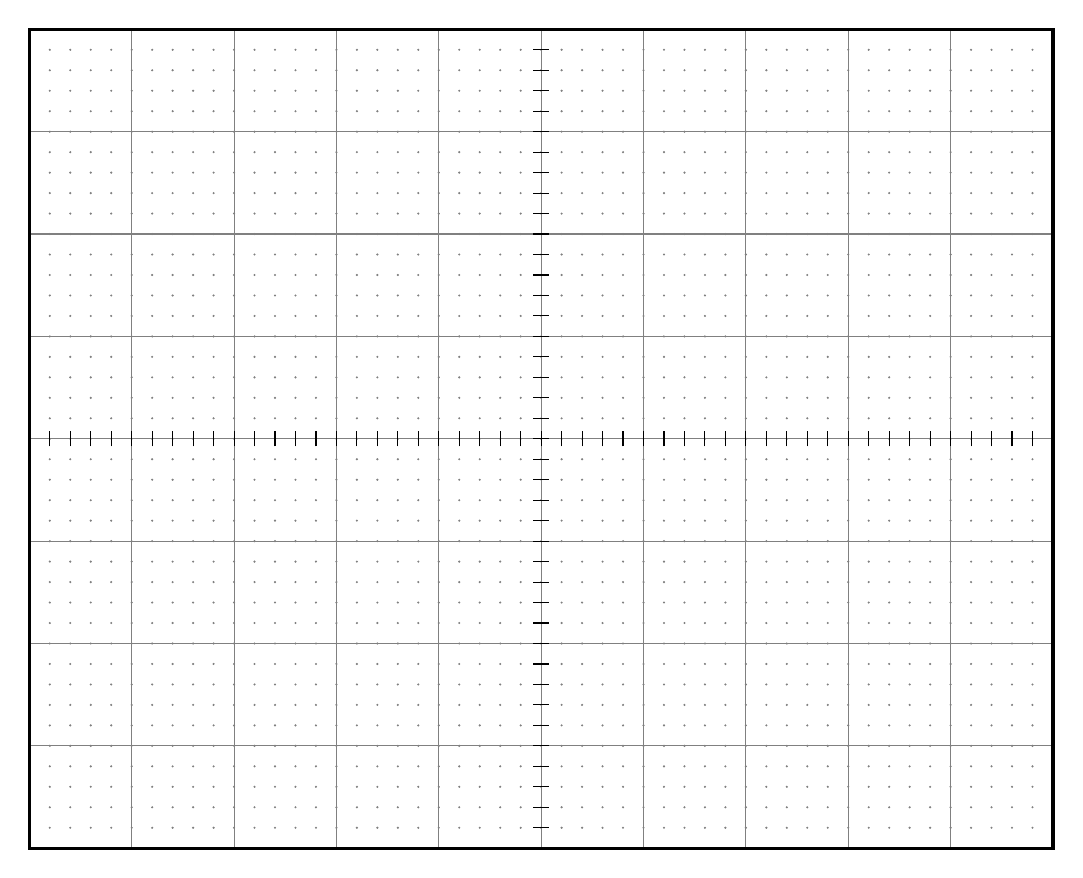
\begin{tikzpicture}
    % Define dimensions
    \def\gridwidth{10}
    \def\gridheight{8}
    \def\spacing{1.3}
    % Draw grid paper on the left
    \begin{scope}[xshift=0cm, yshift=0cm]
        % Grid points
        \foreach \x in {0,2,...,100}
        {
            \foreach \y in {0,2,...,80}
            {
                \draw[gray, fill=gray] (\x*\spacing/10, \y*\spacing/10) circle (0.05mm);
            }
        }
        % Major grid lines
        \foreach \x in {0,1,...,\gridwidth}
            \draw[gray] (\x*\spacing,0) -- (\x*\spacing,\gridheight*\spacing);
        \foreach \y in {0,1,...,\gridheight}
            \draw[gray] (0,\y*\spacing) -- (\gridwidth*\spacing,\y*\spacing);
        \draw[black, very thick] (0,0) rectangle (\gridwidth*\spacing,\gridheight*\spacing);
        % Center gridlines
        \foreach \x in {0,2,...,100}
            \draw (\x*\spacing/10, 3.925*\spacing) -- (\x*\spacing/10, 4.075*\spacing);
        \foreach \y in {0,2,...,80}
            \draw (4.925*\spacing, \y*\spacing/10) -- (5.075*\spacing, \y*\spacing/10);
    \end{scope}
\end{tikzpicture}